\documentclass[a4paper,12pt]{article}

\usepackage[T2A]{fontenc}			
\usepackage[utf8]{inputenc}			
\usepackage[english,russian]{babel}	

\usepackage[
bookmarks=true, colorlinks=true, unicode=true,
urlcolor=black,linkcolor=black, anchorcolor=black,
citecolor=black, menucolor=black, filecolor=black,
]{hyperref}

\usepackage{color}
\usepackage{caption}
\DeclareCaptionFont{white}{\color{black}}
\DeclareCaptionFormat{listing}{\colorbox{white}{\parbox{\textwidth}{#1#2#3}}}
\captionsetup[lstlisting]{format=listing,labelfont=white,textfont=white}

\usepackage{amsmath,amsfonts,amssymb,amsthm,mathtools} 
\usepackage{wasysym}

\usepackage{graphicx}
%\usepackage[cache=false]{minted}
\usepackage{cmap}
\usepackage{indentfirst}

\usepackage{listings} 
\usepackage{fancyvrb}

\usepackage{geometry}
\geometry{left=2cm}
\geometry{right=1.5cm}
\geometry{top=1cm}
\geometry{bottom=2cm}

\usepackage[cache=false]{minted}

\setlength{\parindent}{5ex}
\setlength{\parskip}{0.5em}

\usepackage{pgfplots}
\usetikzlibrary{datavisualization}
\usetikzlibrary{datavisualization.formats.functions}

\begin{document}

	\lstset{ %
		language=C,                 % выбор языка для подсветки (здесь это С)
		basicstyle=\small\sffamily, % размер и начертание шрифта для подсветки кода
		numbers=left,               % где поставить нумерацию строк (слева\справа)
		numberstyle=\tiny,           % размер шрифта для номеров строк
		stepnumber=1,                   % размер шага между двумя номерами строк
		numbersep=5pt,                % как далеко отстоят номера строк от подсвечиваемого кода
		backgroundcolor=\color{white}, % цвет фона подсветки - используем \usepackage{color}
		showspaces=false,            % показывать или нет пробелы специальными отступами
		showstringspaces=false,      % показывать или нет пробелы в строках
		showtabs=false,             % показывать или нет табуляцию в строках
		frame=single,              % рисовать рамку вокруг кода
		tabsize=2,                 % размер табуляции по умолчанию равен 2 пробелам
		captionpos=t,              % позиция заголовка вверху [t] или внизу [b] 
		breaklines=true,           % автоматически переносить строки (да\нет)
		breakatwhitespace=false, % переносить строки только если есть пробел
		escapeinside={\%*}{*)}   % если нужно добавить комментарии в коде
	}
	
	% Титульный лист
	\begin{figure}[h!]
		\begin{center}
			{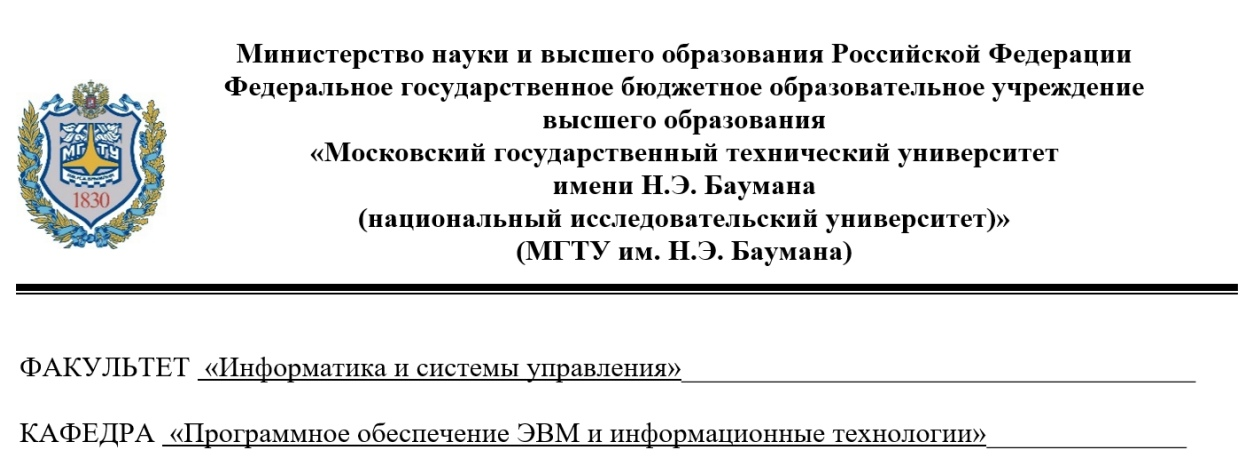
\includegraphics[scale = 0.4]{titul.jpg}}
			\label{titul}
		\end{center}
	\end{figure}
	
	\vspace*{15mm} 
	
	\huge
	\begin{center}
		Дисциплина: <<Операционные системы>>
	\end{center}
	
	\begin{center}
		Лабораторная работа №8
	\end{center}

	
	\huge
	\begin{center}
		Тема работы:\\
		<<Создание виртуальной файловой системы>>
	\end{center}
	\vspace*{30mm} 
	
	\large
	\begin{flushright}
		Студент: Левушкин И. К. \\
		Группа: ИУ7-62Б \\
		Преподаватель: Рязанова Н. Ю. \\
	\end{flushright}
	
	\vspace*{30mm}
	\begin{center}
		Москва, 2020 г.  
	\end{center}
	\thispagestyle{empty}
	
	\newpage
	
	\section*{Создать файловую систему в виде загружаемого модуля ядра, а также slab-кэш для хранения inode созданной файловой системы.}
	
	\section*{Листинг кода программы}
	
	Ниже приведена программа, реализующая поставленную задачу.
	
	\begin{minted}{c}
#include <linux/fs.h>
#include <linux/init.h>
#include <linux/kernel.h>
#include <linux/module.h>
#include <linux/time.h>
#include <linux/slab.h>

static const unsigned long MYFS_MAGIC_NUMBER = 0x13131313;

struct kmem_cache *myfs_cache = NULL;

struct myfs_inode
{
	int i_mode;
	unsigned long i_ino;
};

static void myfs_put_super(struct super_block *sb)
{
    printk(KERN_INFO "MYFS super block destroyed!\n");
}

static int myfs_drop_inode(struct inode *inode)
{
	kmem_cache_free(myfs_cache, inode->i_private);
	return 1;
}

static struct super_operations const myfs_super_ops = {
    .put_super = myfs_put_super,
    .statfs = simple_statfs ,
    .drop_inode = myfs_drop_inode ,
};

static struct inode *myfs_make_inode(struct super_block *sb, int mode)
{
    struct inode *ret = new_inode(sb);

    if (ret) {
        inode_init_owner(ret, NULL, mode); 
        ret->i_size = PAGE_SIZE;
        ret->i_atime = ret->i_mtime = ret->i_ctime = current_time(ret);
	struct myfs_inode *myfs_inode = (struct myfs_inode *)
	kmem_cache_alloc(myfs_cache, GFP_KERNEL);
	myfs_inode->i_mode = ret->i_mode;
	myfs_inode->i_ino = ret->i_ino;
	ret->i_private = myfs_inode;
    }
return ret; 
}

static int myfs_fill_sb(struct super_block *sb, void *data, int silent)
{
    struct inode *root = NULL;

    sb->s_blocksize = PAGE_SIZE; 
    sb->s_blocksize_bits = PAGE_SHIFT;
    sb->s_magic = MYFS_MAGIC_NUMBER;
    sb->s_op = &myfs_super_ops;

    root = myfs_make_inode(sb, S_IFDIR | 0755);
    if (!root)
    {
        printk(KERN_ERR "MYFS inode allocation failed!\n");
       return -ENOMEM;
    }

    root->i_op = &simple_dir_inode_operations; 
    root->i_fop = &simple_dir_operations;

    sb->s_root = d_make_root(root);
    if (!sb->s_root)
    {
        printk(KERN_ERR "MYFS root creation failed!\n");
        return -ENOMEM;
    }

	return 0;
}


static struct dentry *myfs_mount(struct file_system_type *type, 
                                int flags, char const *dev, void *data)
{
    struct dentry *const entry = mount_nodev(type, flags, data, myfs_fill_sb);
    if (IS_ERR(entry))
        printk(KERN_ERR "MYFS mounting failed!\n");
    else
        printk(KERN_DEBUG "MYFS mounted!\n");
    return entry;
}

static struct file_system_type myfs_type = {
    .owner = THIS_MODULE,
    .name = "myfs",
    .mount = myfs_mount,
    .kill_sb = kill_block_super,
    .fs_flags = FS_REQUIRES_DEV, 
};

static int __init myfs_init(void)
{
        int ret = register_filesystem(&myfs_type);
        if (ret != 0)
	{
	    printk(KERN_ERR "MYFS_MODULE cannot register filesystem!\n");
	    return ret;
        }

	myfs_cache = kmem_cache_create("myfs_inode_cache", 
	sizeof(struct myfs_inode), 0, SLAB_POISON, NULL);
	if (!myfs_cache)
	{
		printk(KERN_ERR "kmem_cache_create error\n");
		kmem_cache_destroy(myfs_cache);
		return -ENOMEM;
	}
	printk(KERN_DEBUG "MYFS inode cache created!\n");
    	printk(KERN_DEBUG "MYFS_MODULE loaded\n");
    	return 0;
}

static void __exit myfs_exit(void)
{
	int ret = unregister_filesystem(&myfs_type);

	if (ret != 0)
	{
		printk(KERN_ERR 
		"MYFS_MODULE cannot unregister filesystem!\n");
	}
	else
	{
		kmem_cache_destroy(myfs_cache);
		printk(KERN_DEBUG "MYFS inode cache destroyed!\n");
		printk(KERN_DEBUG "MYFS module unloaded!\n");
	}
}

module_init(myfs_init);
module_exit(myfs_exit);

MODULE_LICENSE("GPL");
MODULE_AUTHOR("Levushkin");
	\end{minted}
	
	\section*{Сценарий сборки программы}
	
	\begin{minted}{make}
ifneq ($(KERNELRELEASE),)
	obj-m := myfs.o

else
	CURRENT = $(shell uname -r)
	KDIR = /lib/modules/$(CURRENT)/build
	PWD = $(shell pwd)

default:
	$(MAKE) -C $(KDIR) M=$(PWD) modules
	sudo make clean

clean:
	rm -rf .tmp_versions
	rm .myfs.*
	#rm *.ko
	rm *.o
	rm *.mod.c
	rm *.symvers
	rm *.order

endif
	\end{minted}
	
	\section*{Демонстрация работы программы}
	
	Ниже представлены загрузка модуля, создание slab-кэша для inode, созданный slab-кэш, создание образа диска, корневой директории и монтирование файловой
	системы:
	
	\begin{figure}[h!]
		\begin{center}
			{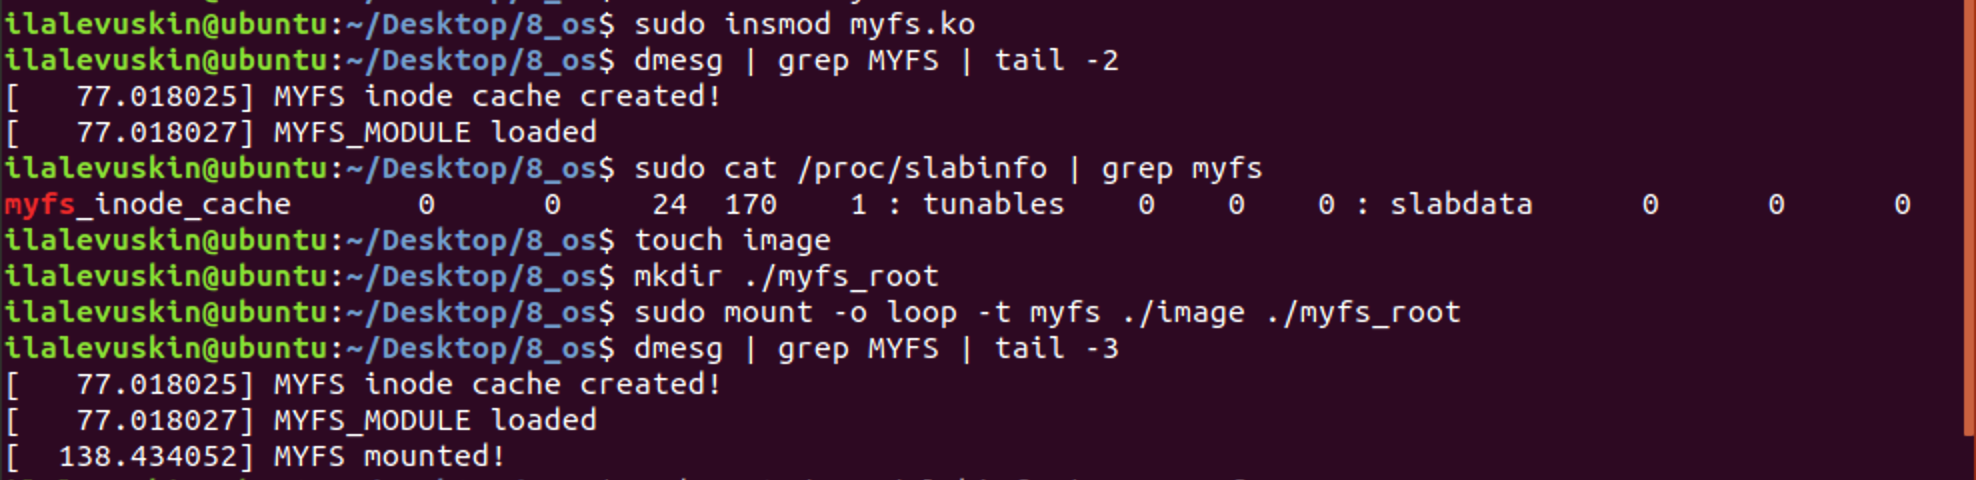
\includegraphics[scale = 0.5]{1.png}}
			\label{1}
		\end{center}
	\end{figure}
	
	 Был создан slab-кэш, содержащий 0 активных объектов, с размером каждого объекта, равным 24 байта.
	 
	 
	 Ниже представлено состояние slab-кэша после монтирования файловой системы:
	 
	 \begin{figure}[h!]
	 	\begin{center}
	 		{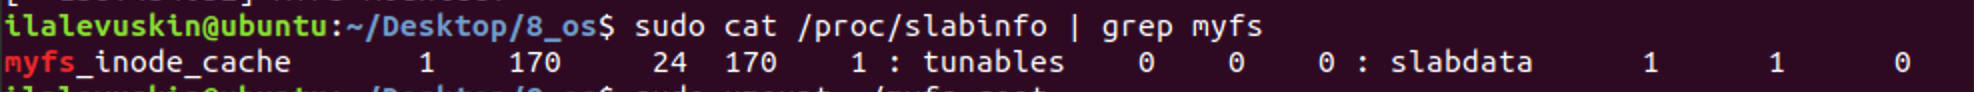
\includegraphics[scale = 0.5]{2.png}}
	 		\label{2}
	 	\end{center}
	 \end{figure}
	 
	 slab-кэш содержит 1 элемент, поскольку при монтировании файловой системы создается inode для корневой директории.
	 
	 \newpage
	 
	 Размонтирование файловой системы и состояние slab-кэша после нее:
	 
	 \begin{figure}[h!]
	 	\begin{center}
	 		{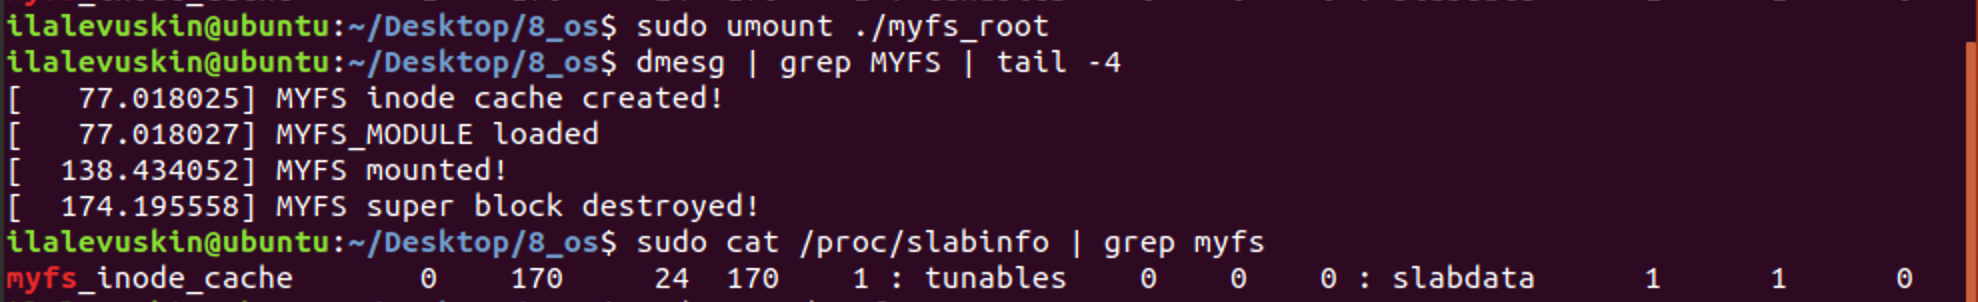
\includegraphics[scale = 0.5]{3.png}}
	 		\label{3}
	 	\end{center}
	 \end{figure}
	 
	 Удаление slab-кэша и выгрузка модуля:
	 
	 \begin{figure}[h!]
	 	\begin{center}
	 		{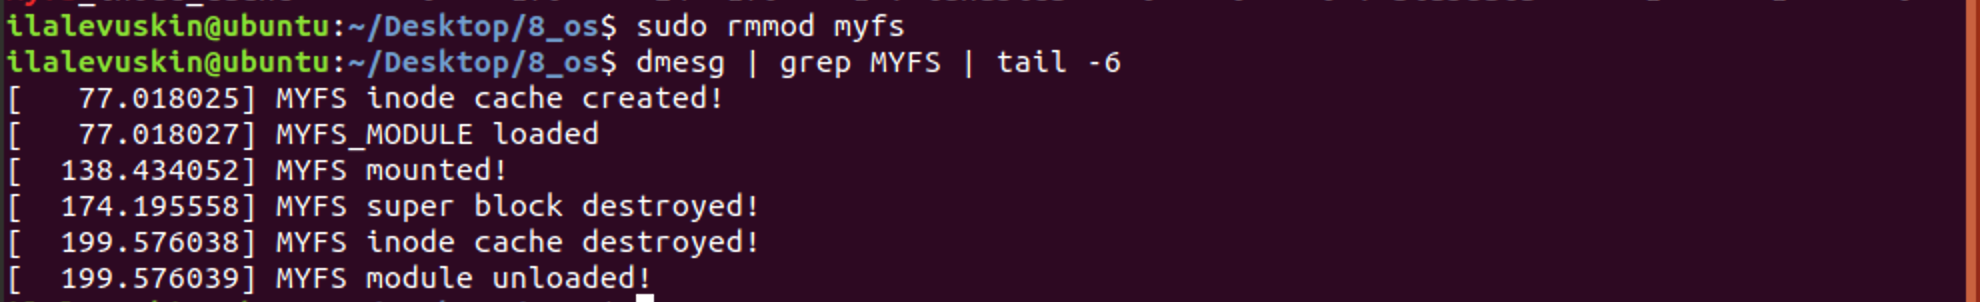
\includegraphics[scale = 0.5]{4.png}}
	 		\label{4}
	 	\end{center}
	 \end{figure}
	 
	
\end{document}